\svnidlong
{$HeadURL$}
{$LastChangedDate$}
{$LastChangedRevision$}
{$LastChangedBy$}
\framebox{Author: \svnauthor; Rev: \svnrev; Last change: \svndate}% - URL: \url{\svnkw{HeadURL}}}
\section{Results}
Results of the aforementioned steps are shown in figure~\ref{fig:wide field scan}. Figure~\ref{subfig:wfs-sub} shows exemplary projection images from overlapping subscans prior to correction and normalization. Figure~\ref{subfig:wfs-mrg} shows a merged projection image prior to reconstruction and figure~\ref{subfig:wfs-slice} shows the end-result of such a wide field scan, a reconstructed slice of the whole sample with a FOV of \unit{5.734}{\milli\meter} --- approximately five times the size of what can be achieved with one single scan.

\begin{figure}[p] % [tb] for small, [p] for big pictures
	\centering
	\begin{minipage}{0.66\textwidth}
	\centering
	\renewcommand{\imsize}{0.2\textwidth}
	\subfloat[Raw projection images from five overlapping subscans. Each image has an original size of 1024$\times$1024 pixels and covers a FOV of approximately \unit{0.7}{\milli\meter}. The images have been rescaled to 512$\times$512 pixels for display purposes.]
	{\label{subfig:wfs-sub}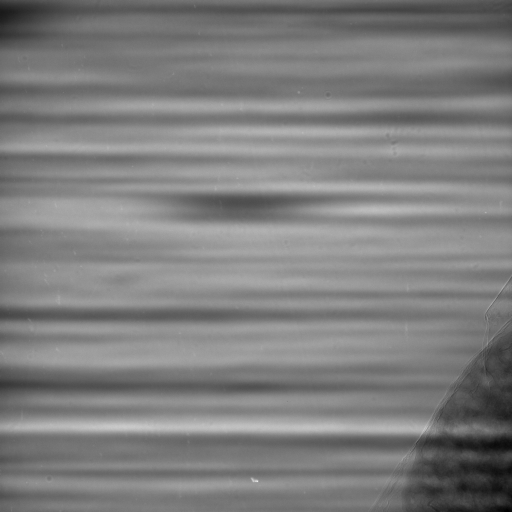
\includegraphics[width=\imsize]{mrg/R108C04BrulW-s10444}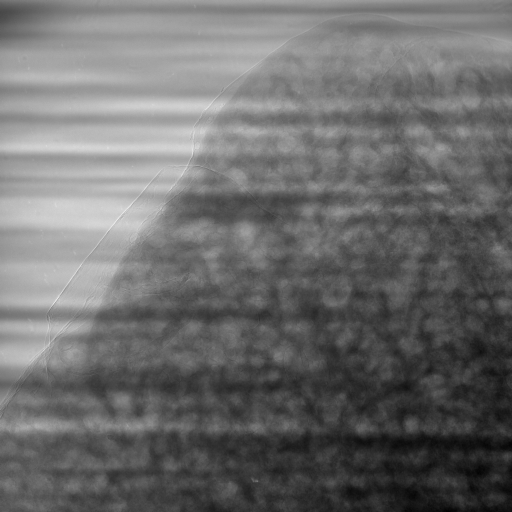
\includegraphics[width=\imsize]{mrg/R108C04BrulW-s20444}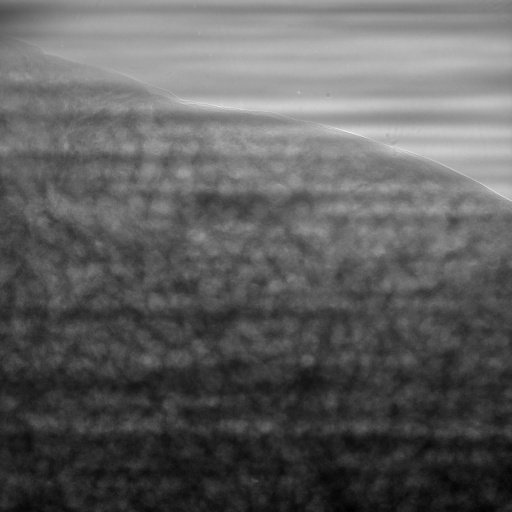
\includegraphics[width=\imsize]{mrg/R108C04BrulW-s30444}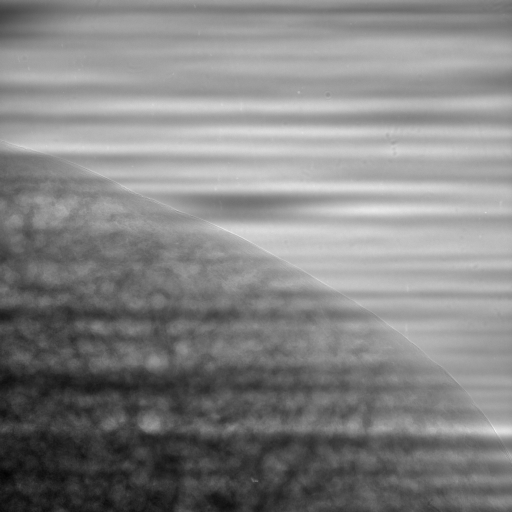
\includegraphics[width=\imsize]{mrg/R108C04BrulW-s40444}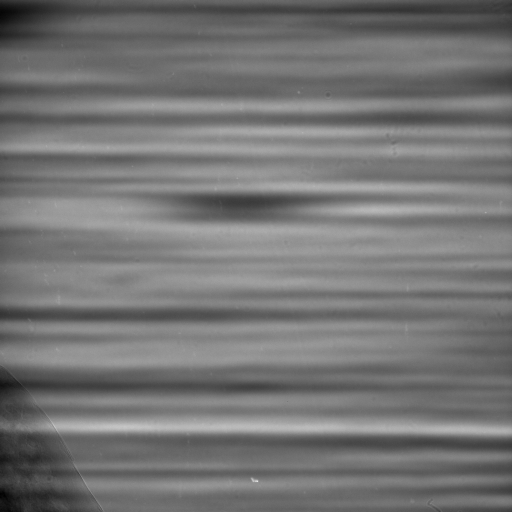
\includegraphics[width=\imsize]{mrg/R108C04BrulW-s50444}}
	\newline
	\renewcommand{\imsize}{\textwidth}
	\subfloat[Merged and corrected projection composed from the subscans shown in \subref{subfig:wfs-sub}. The merged projection has a size of 4502$\times$1024 pixels. The scans shown above overlap each other by 15\%, approximately 150 pixels. A slice reconstructed from a set of merged projections like the one shown here is shown in \subref{subfig:wfs-slice}. The image has been rescaled to 2251$\times$512 pixels for display purposes.]
		{\label{subfig:wfs-mrg}
\includegraphics[width=\imsize]{mrg/R108C04BrulW-cnc0444}}
	\newline
	\subfloat[Reconstructed slice of the full data set with a size of 8192$\times$8192 pixels, covering a FOV of approximately \unit{5.75}{\milli\meter}. The Image has been rescaled to 1024$\times$1024 pixels for display purposes.]
		{\label{subfig:wfs-slice}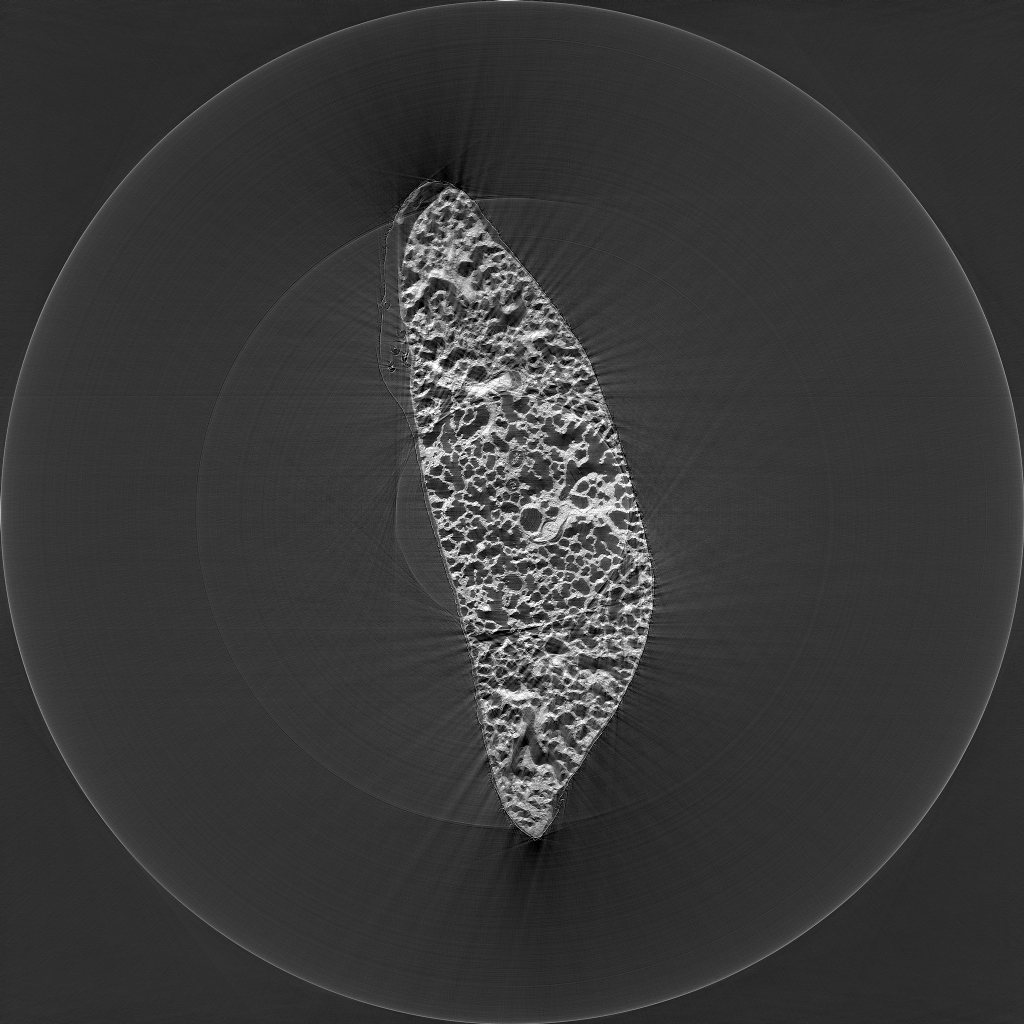
\includegraphics[angle=90,width=\imsize]{R108C04BrulW-1001-mrg-orig}}
	\caption{Different stages of a wide field scan of a sample obtained from a Sprague-Dawley rat 4 days after birth, scanned at a beam energy of \unit{12.6}{\kilo\electronvolt}.}	
	\label{fig:wide field scan}
	\end{minipage}
\end{figure}